\documentclass{article}

% if you need to pass options to natbib, use, e.g.:
%     \PassOptionsToPackage{numbers, compress}{natbib}
% before loading neurips_2020

% ready for submission
% \usepackage{neurips_2020}

% to compile a preprint version, e.g., for submission to arXiv, add add the
% [preprint] option:
%     \usepackage[preprint]{neurips_2020}

% to compile a camera-ready version, add the [final] option, e.g.:
    \usepackage[final]{neurips_2020}

% to avoid loading the natbib package, add option nonatbib:
     % \usepackage[nonatbib]{neurips_2020}

\usepackage[utf8]{inputenc} % allow utf-8 input
\usepackage[T1]{fontenc}    % use 8-bit T1 fonts
\usepackage{hyperref}       % hyperlinks
\usepackage{url}            % simple URL typesetting
\usepackage{booktabs}       % professional-quality tables
\usepackage{amsfonts}       % blackboard math symbols
\usepackage{nicefrac}       % compact symbols for 1/2, etc.
\usepackage{microtype}      % microtypography

%% Customized package by Mao Song
\usepackage{listings}
\usepackage{graphicx}
\usepackage{amsthm}
\usepackage{amsmath}
\newcommand*\diff{\mathop{}\!\mathrm{d}}
\theoremstyle{definition}
\newtheorem{solution}{Solution}

\usepackage{xcolor}

\definecolor{codegreen}{rgb}{0,0.6,0}
\definecolor{codegray}{rgb}{0.5,0.5,0.5}
\definecolor{codepurple}{rgb}{0.58,0,0.82}
\definecolor{backcolour}{rgb}{0.95,0.95,0.92}

\lstdefinestyle{mystyle}{
    backgroundcolor=\color{backcolour},   
    commentstyle=\color{codegreen},
    keywordstyle=\color{magenta},
    numberstyle=\tiny\color{codegray},
    stringstyle=\color{codepurple},
    basicstyle=\ttfamily\footnotesize,
    breakatwhitespace=false,         
    breaklines=true,                 
    captionpos=b,                    
    keepspaces=true,                 
    numbers=left,                    
    numbersep=5pt,                  
    showspaces=false,                
    showstringspaces=false,
    showtabs=false,                  
    tabsize=2
}

\lstset{style=mystyle}


\title{Homework 3 for SI211: Numerical Analysis}

% The \author macro works with any number of authors. There are two commands
% used to separate the names and addresses of multiple authors: \And and \AND.
%
% Using \And between authors leaves it to LaTeX to determine where to break the
% lines. Using \AND forces a line break at that point. So, if LaTeX puts 3 of 4
% authors names on the first line, and the last on the second line, try using
% \AND instead of \And before the third author name.

\author{%
  {Mao Song} \\
  SIST\\
  ShanghaiTech University\\
  Student ID: 2019233134 \\
  \texttt{maosong@shanghaitech.edu.cn} \\
}

\begin{document}

\maketitle

\begin{abstract}
  This is the solution for Homework 3 of SI211: Numerical Analysis, which is taught by Boris Houska.
\end{abstract}

\section{Natural Spline}
Write a computer code in Julia, Matlab, Python, C++, (or a similar programming language), which returns a natural spline that  interpolates the function $f:[x_0, x_N]\to\mathbb{R}$ the equidistantpoints
\begin{equation}
	\forall i\in\{0,1,\dots,N\},x_i=x_0+hi
\end{equation}
where 
\begin{equation}
	h = \frac{x_N-x_0}{N}
\end{equation}
\begin{solution}
  	The Matlab code is listed as follows:
  	\begin{lstlisting}[language=Matlab]
function [a, b, c, d] = natual_spline(x0, xN, N, init_func)
  %%%%%%%%%%%%%%%%%%%%%%%%%%%%%%%%%
  % This function aims to implement the algorithm 3.4:
  % Natural Cubic Spline in <<Numerical Anslysis>> 9th.
  % But with a interval [x0, xN] and a fix length h of subinterval
  % that is, x_i = x0 + i*h

  % Parameters:
  %   x0: left endpoint of the interval
  %   xN: right endpoint of the interval
  %   N: The number of intervals in [x0, xN]
  %   init_func: function handle
  %             the function we need to interpolate

  % Return
  %   a, b, c, d: an array-like, shape=[N, 1]
  %       the cubic spline function coefficient in each subinterval 
  %           [x_i,x_{i+1}]
  %%%%%%%%%%%%%%%%%%%%%%%%%%%%%%%%%

  % step 1
  h = (xN - x0) / N;
  x = x0: h: xN;
  a = init_func(x);
  % step 2
  alpha = 3/h * (a(3:end) - 2 * a(2:end-1) + a(1:end-2));

  % Use Theorem 3.11 to solve c
  % the coefficient matrix
  A = diag(4*h*ones(N-1, 1)) + diag(h*ones(N-2, 1), 1) + diag(h*ones(N-2, 1), -1);
  c = (A\alpha')';
  c = [0, c, 0];

  % step 6
  b = (a(2:end) - a(1:end-1)) / h - h/3 * (c(2:end) + 2*c(1:end-1));
  d = (c(2:end) - c(1:end-1)) / (3 * h);
end
\end{lstlisting}
\end{solution}



\section{Comparision of Interpolation and Natural Spline}
We have constructed a computer program that interpolates a function $f(x) =1/(1+x^2)$ with a polynomialof order $10$. Use your code from the first exercise to interpolates this function 
\begin{equation}
	f(x) =\frac{1}{1+x^2}
\end{equation}
 at the points $x_1=-5, x_2=-4, x_3=-3,\dots, x_{10}= 4, x_{11}= 5$. Plot the functionf as well as the natural spline that interpolates $f$ and the interpolating polynomials (HW2).


\begin{solution}
	As figure \ref{Fig:solution_to_problem3} shows, the natural spline approximates the function $f$ extremely well, while the Lagrange interpolation polynomial performance badlly when the $x$ is far away from $0$.
	\begin{figure}[ht]
      \label{Fig:solution_to_problem3}
      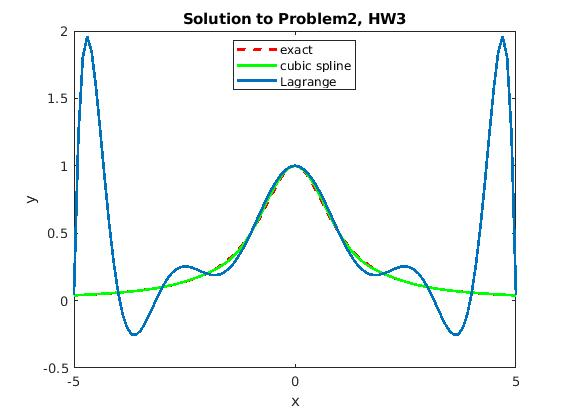
\includegraphics[width=0.8\textwidth]{solution_to_problem2.jpg}
      \centering
      \caption{The interpolation for $f(x)=1/(1+x^2)$}
    \end{figure}
\end{solution}




\section{Comparision of Interpolation and Natural Spline (continued)}
For the function $f$, the interpolating polynomial $p$, and the interpolating spline $s$ from the previous exercise, compute
\begin{enumerate}
	\item the value of the integral
	\begin{equation}
		\int_{-5}^{5}\left[f''(x)\right]^2\diff x
	\end{equation}
	\item the value of the integral
	\begin{equation}
		\int_{-5}^{5}\left[p''(x)\right]^2\diff x
	\end{equation}
	\item the value of the integral
	\begin{equation}
		\int_{-5}^{5}\left[s''(x)\right]^2\diff x
	\end{equation}
\end{enumerate}
Interpret your results.



\begin{solution}
    \begin{enumerate}
    	\item Since 
    	\begin{equation}
    		f'(x)=-\frac{2x}{(1+x^2)^2},\quad  f''(x)=\frac{8x^2-2(1+x^2)}{(1+x^2)^3}
    	\end{equation}
    	Thus
    	\begin{align*}
    	\int_{-5}^{5}\left[f''(x)\right]^2\diff x&=\int_{-5}^{5}\left[\frac{8x^2-2(1+x^2)}{(1+x^2)^3}\right]^2\diff x\\
    	&=\frac{1}{20}\left[\frac{x (15 x^8 + 70 x^6 + 128 x^4 + 10 x^2 + 65)}{(x^2 + 1)^5}+15 \arctan(x)\right]_{-5}^5\\
    	&=\frac{219795}{742586} + \frac32 \arctan(5)\\
    	&\approx 2.3561
    	\end{align*}

    	\item Since 
    	\begin{equation}
    		p(x)=\sum_{k=0}^Nf(x_k)\prod_{i=0,i\neq k}^{N}\frac{(x-x_i)}{(x_k-x_i)}
    	\end{equation}
    	We use the Matlab \emph{diff} and \emph{int} function to calculate the result, the code is in \emph{solution\_to\_problem\_3.m}. The result is
    	\begin{equation}
    		\int_{-5}^{5}\left[p''(x)\right]^2\diff x\approx 2007.70
    	\end{equation}
    	
    	\item Since 
    	\begin{equation}
    		s(x)=s_i(x), x\in[-6+i,-5+i], \quad i=1,\dots,10
    	\end{equation}
    	where $s_i(x)=a_i+b_i(x-x_i)+c_i(x-x_i)^2+d_i(x-x_i)^3$. 
    	we have
    	\begin{align*}
    		\int_{-5}^{5}\left[s''(x)\right]^2\diff x&=\sum_{i=1}^{10}\int_{-6+i}^{-5+i}\left[s_i''(x)\right]^2\diff x\\
    		&=\sum_{i=1}^{10}\int_{-6+i}^{-5+i}\left[2c_i+6d_i(x-x_i)\right]^2\diff x\\
    		&=4\sum_{i=1}^{10}c_i^2+12\sum_{i=1}^{10}c_id_i+12\sum_{i=1}^{10}d_i^2\\
    		&\approx2.2161
    	\end{align*}
    	where in the last step we use the numerical result computed by Problem 2.
    \end{enumerate}
    \textbf{Interpretation}: 
    \begin{enumerate}
    	\item  The natural cubic spline $s$ never oscillates more than the function $f$.  That is,
    	\begin{equation}
    		\int_{x_0}^{x_N}[s''(x)]^2\diff x\leq \int_{x_0}^{x_N}[f''(x)]^2\diff x
    	\end{equation}
    	\item High order interpolating polynomials tends to oscillate ``unreasonably''.

    \end{enumerate}
    

    
\end{solution}





\end{document}
